% ============================================================
%  Red/Blue Team 실습 환경 — 내부 공유용
%  이선우 (KENTECH STIS Lab)
% ============================================================
\documentclass[aspectratio=169,10pt]{beamer}
\usetheme{metropolis}
\setbeamertemplate{navigation symbols}{}
\setbeamertemplate{footline}[frame number]
\setbeamercolor{frametitle}{bg=black!85,fg=white}
\setbeamercolor{progress bar}{fg=orange!80!black}
\setbeamerfont{itemize/enumerate body}{size=\footnotesize}
\setbeamerfont{itemize/enumerate subbody}{size=\scriptsize}
\setbeamerfont{block body}{size=\footnotesize}
\setbeamerfont{block title}{size=\small}

\usepackage{kotex}
\setmainfont{Noto Sans CJK KR}[BoldFont={Noto Sans CJK KR Bold}]
\setsansfont{Noto Sans CJK KR}[BoldFont={Noto Sans CJK KR Bold}]
\setmonofont{Noto Sans Mono CJK KR}[Scale=0.85]
\setmainhangulfont{Noto Sans CJK KR}[BoldFont={Noto Sans CJK KR Bold}]
\setsanshangulfont{Noto Sans CJK KR}[BoldFont={Noto Sans CJK KR Bold}]
\usepackage{tikz}
\usetikzlibrary{positioning,calc,arrows.meta,shapes.geometric,
                 decorations.pathreplacing,backgrounds,fit}
\usepackage{pgfplots}
\pgfplotsset{compat=1.16}
\usepackage{booktabs,listings,xcolor,adjustbox,colortbl,multicol}

\makeatletter
\@ifundefined{tikzscope@linewidth}{\newdimen\tikzscope@linewidth}{}
\@ifundefined{pgfscope@linewidth}{\newdimen\pgfscope@linewidth}{}
\@ifundefined{pgfsys@end@save}{\def\pgfsys@end@save{\pgfsys@endscope}}{}
\makeatother

\definecolor{coreBlue}{RGB}{50,100,170}
\definecolor{intGreen}{RGB}{60,140,80}
\definecolor{opsOrange}{RGB}{200,120,50}
\definecolor{accent}{RGB}{200,60,60}
\definecolor{muted}{RGB}{120,120,120}
\definecolor{codegreen}{RGB}{0,120,0}
\definecolor{redTeam}{RGB}{190,40,40}
\definecolor{blueTeam}{RGB}{30,80,170}
\definecolor{layer1}{RGB}{220,232,245}
\definecolor{layer2}{RGB}{225,240,225}
\definecolor{layer3}{RGB}{245,230,220}
\definecolor{juiceGreen}{RGB}{80,160,50}
\definecolor{dashBg}{RGB}{13,17,23}

\lstdefinestyle{code}{
  basicstyle=\ttfamily\scriptsize,
  keywordstyle=\color{coreBlue}\bfseries,
  commentstyle=\color{muted},
  stringstyle=\color{codegreen},
  showstringspaces=false, breaklines=true,
  frame=single, rulecolor=\color{muted!40},
  xleftmargin=4pt, aboveskip=4pt, belowskip=4pt,
  escapeinside={(*@}{@*)},
}
\lstset{style=code}
\newcommand{\hlt}[1]{\textcolor{accent}{\textbf{#1}}}
\newcommand{\red}[1]{\textcolor{redTeam}{\textbf{#1}}}
\newcommand{\blue}[1]{\textcolor{blueTeam}{\textbf{#1}}}

\title{Red/Blue Team 실시간 공격·방어 실습 환경}
\subtitle{OWASP Juice Shop + Docker Compose + Suricata + Web Dashboard}
\author{이선우}
\institute{KENTECH STIS Lab}
\date{\today}

\begin{document}

\maketitle

% ============================================================
\section{뭘 만들었는가}
% ============================================================

\begin{frame}{한 줄 요약}
\begin{center}
\Large
\texttt{bash start.sh} 한 번이면\\[0.3em]
\hlt{공격 12종} + \blue{IDS 탐지 11종} + \hlt{웹 대시보드}가\\[0.3em]
로컬에서 즉시 동작하는 실습 환경
\end{center}

\vspace{1em}
\begin{columns}[T]
\begin{column}{0.48\textwidth}
\begin{block}{Red Team (공격)}
\begin{itemize}
    \item SQLi, XSS, Brute Force (Web/SSH/FTP)
    \item Bot, DoS, PortScan, Infiltration
    \item 버튼 클릭으로 PoC 실행
    \item 학생이 새 PoC 추가 가능
\end{itemize}
\end{block}
\end{column}
\begin{column}{0.48\textwidth}
\begin{block}{Blue Team (방어)}
\begin{itemize}
    \item Suricata IDS 규칙 11종 preset
    \item 규칙 ON/OFF 토글
    \item 실시간 탐지 결과 모니터링
    \item 학생이 새 규칙 추가 가능
\end{itemize}
\end{block}
\end{column}
\end{columns}
\end{frame}

% ============================================================
\section{전체 아키텍처}
% ============================================================

\begin{frame}{시스템 아키텍처 — Docker Compose 8개 서비스}
\begin{center}
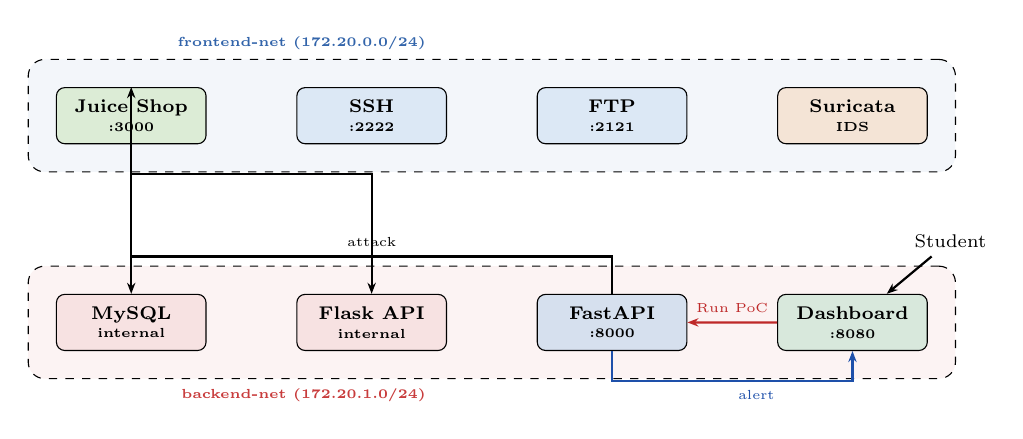
\begin{tikzpicture}[
    svc/.style={draw, rounded corners=3pt, minimum width=2cm, minimum height=0.75cm, font=\scriptsize\bfseries, align=center},
    net/.style={draw, dashed, rounded corners=6pt, inner sep=10pt},
    arr/.style={-{Stealth[length=4pt]}, thick},
    scale=0.95, transform shape,
]
% Frontend row
\node[svc, fill=juiceGreen!20] (js) {Juice Shop\\[-1pt]{\tiny :3000}};
\node[svc, fill=layer1, right=1.2cm of js] (ssh) {SSH\\[-1pt]{\tiny :2222}};
\node[svc, fill=layer1, right=1.2cm of ssh] (ftp) {FTP\\[-1pt]{\tiny :2121}};
\node[svc, fill=opsOrange!20, right=1.2cm of ftp] (sur) {Suricata\\[-1pt]{\tiny IDS}};

% Backend row - more spacing
\node[svc, fill=accent!15, below=2cm of js] (db) {MySQL\\[-1pt]{\tiny internal}};
\node[svc, fill=accent!15, right=1.2cm of db] (api) {Flask API\\[-1pt]{\tiny internal}};
\node[svc, fill=coreBlue!20, right=1.2cm of api] (back) {FastAPI\\[-1pt]{\tiny :8000}};
\node[svc, fill=intGreen!20, right=1.2cm of back] (dash) {Dashboard\\[-1pt]{\tiny :8080}};

% Network boxes
\begin{scope}[on background layer]
\node[net, fill=coreBlue!6, fit=(js)(ssh)(ftp)(sur), label={[font=\tiny\bfseries,coreBlue]above left:frontend-net (172.20.0.0/24)}] {};
\node[net, fill=accent!6, fit=(db)(api)(back)(dash), label={[font=\tiny\bfseries,accent]below left:backend-net (172.20.1.0/24)}] {};
\end{scope}

% Arrows - spread out
\draw[arr] (js) -- (db);
\draw[arr] (js.south) -- ++(0,-0.4) -| (api);
\draw[arr] (back.north) -- ++(0,0.5) -| node[above, font=\tiny, pos=0.25] {attack} (js.north);
\draw[arr, redTeam] (dash.west) -- node[above, font=\tiny] {Run PoC} (back.east);
\draw[arr, blueTeam] (back.south) -- ++(0,-0.4) -| node[below, font=\tiny, pos=0.3] {alert} (dash.south);

% User
\node[font=\scriptsize, above right=0.5cm and -0.3cm of dash] (user) {Student};
\draw[arr] (user) -- (dash);
\end{tikzpicture}
\end{center}

\vspace{0.2em}
{\scriptsize
\red{Red}: Dashboard $\rightarrow$ FastAPI $\rightarrow$ PoC 실행 $\rightarrow$ Juice Shop/SSH/FTP 공격 \quad
\blue{Blue}: 공격 탐지 $\rightarrow$ eve.json $\rightarrow$ Dashboard 실시간 표시
}
\end{frame}

% ============================================================
\begin{frame}{데이터 흐름 — 공격부터 탐지까지}
\begin{tikzpicture}[
    flowbox/.style={draw, rounded corners=3pt, minimum width=2.8cm, minimum height=0.7cm, font=\small, align=center},
    arr/.style={-{Stealth[length=5pt]}, thick},
]
\node[flowbox, fill=redTeam!15] (s1) {1. Run 버튼 클릭};
\node[flowbox, fill=coreBlue!15, right=0.8cm of s1] (s2) {2. FastAPI\\PoC 실행};
\node[flowbox, fill=juiceGreen!15, right=0.8cm of s2] (s3) {3. 공격 트래픽\\발생};
\node[flowbox, fill=opsOrange!15, below=0.8cm of s3] (s4) {4. Alert 기록\\eve.json};
\node[flowbox, fill=blueTeam!15, left=0.8cm of s4] (s5) {5. Dashboard\\실시간 표시};
\node[flowbox, fill=intGreen!15, left=0.8cm of s5] (s6) {6. 통계 차트\\업데이트};

\draw[arr] (s1) -- (s2);
\draw[arr] (s2) -- (s3);
\draw[arr] (s3) -- (s4);
\draw[arr] (s4) -- (s5);
\draw[arr] (s5) -- (s6);
\end{tikzpicture}

\vspace{0.5em}
\begin{columns}[T]
\begin{column}{0.48\textwidth}
\begin{block}{Backend (FastAPI)}
\begin{itemize}
    \item \texttt{POST /api/attacks/\{id\}/run}
    \item subprocess로 Python/Bash PoC 실행
    \item 결과 stdout/stderr 반환
    \item 실행 후 eve.json에 alert 자동 기록
\end{itemize}
\end{block}
\end{column}
\begin{column}{0.48\textwidth}
\begin{block}{Monitor (3초 폴링)}
\begin{itemize}
    \item \texttt{GET /api/alerts} 3초 간격 폴링
    \item 공격 완료 직후 즉시 리로드
    \item 새로고침 없이 실시간 반영
    \item 공격 유형별 통계 차트
\end{itemize}
\end{block}
\end{column}
\end{columns}
\end{frame}

% ============================================================
\section{Juice Shop 확장}
% ============================================================

\begin{frame}{OWASP Juice Shop — 원본 vs 우리 환경}
\begin{columns}[T]
\begin{column}{0.48\textwidth}
\begin{block}{Juice Shop 원본 (그대로 사용)}
\begin{itemize}
    \item 공식 이미지 \texttt{bkimminich/juice-shop}
    \item 소스코드 수정 없음
    \item 기존 취약점 그대로 활용:
    \begin{itemize}
        \item SQLi (로그인, 검색)
        \item XSS (DOM, Reflected, Stored)
        \item 인증 없는 API endpoints
    \end{itemize}
\end{itemize}
\end{block}
\end{column}
\begin{column}{0.48\textwidth}
\begin{block}{\hlt{Docker Compose로 추가한 것}}
\begin{itemize}
    \item \textbf{SSH 서버} — Brute Force 대상\\
          {\scriptsize admin/admin123, port 2222}
    \item \textbf{FTP 서버} — Brute Force 대상\\
          {\scriptsize admin/admin123, secret.txt}
    \item \textbf{Internal DB} — Infiltration 대상\\
          {\scriptsize MySQL, FLAG\{...\} 테이블}
    \item \textbf{Internal API} — 내부망 피벗\\
          {\scriptsize Flask, /admin/users endpoint}
    \item \textbf{Suricata} — IDS 탐지 엔진
    \item \textbf{FastAPI} — PoC 실행 + 규칙 관리
    \item \textbf{Dashboard} — React 웹 UI
\end{itemize}
\end{block}
\end{column}
\end{columns}
\end{frame}

% ============================================================
\begin{frame}{네트워크 설계 — 왜 이렇게 나눴는가}
\begin{columns}[T]
\begin{column}{0.50\textwidth}
\begin{tikzpicture}[
    svc/.style={draw, rounded corners=2pt, minimum width=1.6cm, minimum height=0.55cm, font=\scriptsize\bfseries, align=center},
    net/.style={draw, dashed, rounded corners=4pt, inner sep=6pt},
    arr/.style={-{Stealth[length=3pt]}, thick},
]
% Frontend
\node[svc, fill=juiceGreen!20] (js) {Juice Shop};
\node[svc, fill=layer1, right=0.8cm of js] (ssh) {SSH};
\node[svc, fill=layer1, right=0.8cm of ssh] (ftp) {FTP};

% Backend - more vertical space
\node[svc, fill=accent!15, below=1.8cm of js] (db) {MySQL};
\node[svc, fill=accent!15, right=0.8cm of db] (api) {Flask};

% Network labels
\begin{scope}[on background layer]
\node[net, fill=coreBlue!6, fit=(js)(ssh)(ftp), label={[font=\tiny\bfseries,coreBlue]above:frontend-net}] {};
\node[net, fill=accent!6, fit=(db)(api), label={[font=\tiny\bfseries,accent]below:backend-net}] {};
\end{scope}

% Arrows
\draw[arr] (js) -- node[left, font=\tiny] {양쪽 연결} (db);
\draw[arr] (js.south) -- ++(0,-0.5) -| (api);
\draw[arr, redTeam, dashed] ([xshift=3pt]js.south) -- ++(0,-0.7) -| node[right, font=\tiny, pos=0.3] {Infiltration} ([xshift=3pt]db.north);

\node[font=\tiny, muted, right=0.4cm of ftp] {학생 접근};
\node[font=\tiny, accent, right=0.4cm of api] {외부 차단};
\end{tikzpicture}
\end{column}
\begin{column}{0.46\textwidth}
\begin{alertblock}{핵심 설계 의도}
\begin{itemize}
    \item frontend-net: 학생이 직접 접근
    \item backend-net: \hlt{외부 비노출}
    \item Juice Shop만 양쪽 연결
    \item Infiltration: 웹앱 취약점으로\\내부망 도달하는 시나리오
\end{itemize}
\end{alertblock}
\end{column}
\end{columns}
\end{frame}

% ============================================================
\section{공격 PoC 12종}
% ============================================================

\begin{frame}{사전 준비된 공격 PoC — 12종}
\begin{adjustbox}{max width=\textwidth}
\footnotesize
\begin{tabular}{llllll}
\toprule
\textbf{ID} & \textbf{이름} & \textbf{유형} & \textbf{대상} & \textbf{언어} & \textbf{CIC-IDS Label} \\
\midrule
\rowcolor{layer3} sqli\_login\_bypass & 로그인 우회 & SQLi & Juice Shop & Python & Web Attack -- Sql Injection \\
\rowcolor{layer3} sqli\_union\_select & UNION SELECT & SQLi & Juice Shop & Python & Web Attack -- Sql Injection \\
\rowcolor{layer3} xss\_dom & DOM XSS & XSS & Juice Shop & Python & Web Attack -- XSS \\
\rowcolor{layer3} xss\_reflected & Reflected XSS & XSS & Juice Shop & Python & Web Attack -- XSS \\
\rowcolor{layer3} xss\_stored & Stored XSS & XSS & Juice Shop & Python & Web Attack -- XSS \\
\rowcolor{layer3} brute\_web & Web 로그인 BF & BruteForce & Juice Shop & Python & Web Attack -- Brute Force \\
\rowcolor{layer1} brute\_ssh & SSH BF & BruteForce & SSH 서버 & Bash & SSH-Patator \\
\rowcolor{layer1} brute\_ftp & FTP BF & BruteForce & FTP 서버 & Bash & FTP-Patator \\
\rowcolor{layer2} bot\_scraper & 자동 스크래핑 & Bot & Juice Shop & Python & Bot \\
\rowcolor{layer2} dos\_slowloris & Slowloris & DoS & Juice Shop & Python & DoS slowloris \\
\rowcolor{layer2} portscan & 네트워크 스캔 & PortScan & Docker net & Bash & PortScan \\
\rowcolor{layer3} infiltration & 내부망 침투 & Infiltration & Internal & Python & Infiltration \\
\bottomrule
\end{tabular}
\end{adjustbox}
\vspace{0.3em}

{\footnotesize \colorbox{layer3}{\strut Web App 대상} \quad \colorbox{layer1}{\strut 인프라 대상} \quad \colorbox{layer2}{\strut 네트워크 대상} \quad 모두 대시보드에서 버튼 클릭으로 실행}
\end{frame}

% ============================================================
\section{IDS 규칙 11종}
% ============================================================

\begin{frame}{Suricata 탐지 규칙 — 11종 Preset}
\begin{adjustbox}{max width=\textwidth}
\footnotesize
\begin{tabular}{rlll}
\toprule
\textbf{SID} & \textbf{탐지 대상} & \textbf{시그니처 핵심} & \textbf{대응 공격} \\
\midrule
100001 & SQLi Attempt & \texttt{SELECT} + \texttt{'}/\texttt{--}/\texttt{\#} in URI & sqli\_login\_bypass \\
100002 & SQLi UNION & \texttt{UNION}+\texttt{SELECT} in URI & sqli\_union\_select \\
100003 & XSS Script Tag & \texttt{<script} in HTTP & xss\_* \\
100004 & XSS Event Handler & \texttt{onload|onerror} pattern & xss\_* \\
100005 & Web Brute Force & POST /rest/user/login $\times$5/30s & brute\_web \\
100006 & SSH Brute Force & port 2222 SYN $\times$5/60s & brute\_ssh \\
100007 & FTP Brute Force & port 21 USER $\times$5/60s & brute\_ftp \\
100008 & Bot Scraping & GET /api/Products $\times$30/10s & bot\_scraper \\
100009 & DoS Slowloris & SYN $\times$20/10s to HTTP & dos\_slowloris \\
100010 & Port Scan & SYN $\times$20/5s multi-port & portscan \\
100011 & Infiltration & frontend $\rightarrow$ MySQL (3306) & infiltration \\
\bottomrule
\end{tabular}
\end{adjustbox}
\vspace{0.3em}

{\footnotesize 모든 규칙은 대시보드에서 \blue{ON/OFF 토글} 가능. 학생이 \hlt{새 규칙 추가}도 가능 (SID 200000\textasciitilde).}
\end{frame}

% ============================================================
\section{웹 대시보드}
% ============================================================

\begin{frame}{대시보드 — 3-Panel 레이아웃}
\begin{tikzpicture}[
    panel/.style={draw, rounded corners=3pt, minimum height=3.5cm, font=\footnotesize, align=left, text width=3.5cm},
    term/.style={draw, rounded corners=3pt, minimum height=1cm, font=\footnotesize, align=left},
]
% Panels
\node[panel, fill=redTeam!8, text=redTeam] (atk) at (0,0) {
    \textbf{Attack Panel}\\[3pt]
    {[}+ New Attack{]}\\[2pt]
    --- Preset (12) ---\\
    $\square$ SQLi Login {[}Run{]}\\
    $\square$ XSS DOM {[}Run{]}\\
    $\square$ Brute SSH {[}Run{]}\\
    ...\\[2pt]
    --- Custom ---\\
    $\square$ My Attack {[}Edit{]}
};
\node[panel, fill=blueTeam!8, text=blueTeam, right=0.3cm of atk] (def) {
    \textbf{Defense Panel}\\[3pt]
    {[}+ New Rule{]} {[}Reload{]}\\[2pt]
    --- Preset (11) ---\\
    $[\bullet]$ SQLi Detect\\
    $[\bullet]$ XSS Detect\\
    $[\circ]$ BF Detect (OFF)\\
    ...\\[2pt]
    --- Custom ---\\
    $[\bullet]$ My Rule
};
\node[panel, fill=intGreen!8, right=0.3cm of def, text width=4cm] (mon) {
    \textbf{Live Monitor}\\[3pt]
    {[}Feed{]} {[}Stats{]} {[}System{]}\\[2pt]
    07:41:37 \red{HIGH}\\
    \quad SQLi Detected\\
    07:41:38 \red{HIGH}\\
    \quad XSS Detected\\
    07:42:01 \textcolor{opsOrange}{MED}\\
    \quad Bot Activity\\[2pt]
    \textcolor{muted}{\scriptsize 3초 자동 폴링}
};

% Terminal
\node[term, fill=dashBg, text=white, text width=12.3cm, below=0.2cm of def, font=\ttfamily\scriptsize] (trm) {
    \textcolor{coreBlue}{[run]} Starting "SQLi Login Bypass"...\\
    \textcolor{intGreen}{[+]} SUCCESS! Auth Token: eyJ0eX...\\
    \textcolor{coreBlue}{[run]} Completed. \quad\quad\quad\quad \textcolor{muted}{drag handle $\updownarrow$}
};

% Header
\node[font=\small\bfseries, above=0.1cm of def] {Red/Blue Team Lab \quad\quad \textcolor{intGreen}{$\bullet$} WS Connected};
\end{tikzpicture}
\end{frame}

% ============================================================
\begin{frame}{대시보드 — 핵심 기능 상세}
\begin{columns}[T]
\begin{column}{0.48\textwidth}
\begin{block}{\red{Attack Panel} 기능}
\begin{itemize}
    \item Preset 12종 PoC 목록
    \item \texttt{[View Code]} — 소스코드 모달
    \item \texttt{[Run]} — 즉시 실행, Terminal에 결과
    \item \texttt{[+ New Attack]} — Monaco Editor\\
          Python/Bash 선택, 저장 즉시 반영
    \item Custom은 편집/삭제 가능
\end{itemize}
\end{block}
\vspace{0.3em}
\begin{block}{Terminal}
\begin{itemize}
    \item 공격 실행 stdout/stderr 표시
    \item 드래그로 상하 크기 조절
    \item Clear 버튼
\end{itemize}
\end{block}
\end{column}
\begin{column}{0.48\textwidth}
\begin{block}{\blue{Defense Panel} 기능}
\begin{itemize}
    \item Preset 11종 Suricata 규칙
    \item \texttt{ON/OFF} 토글 — 즉시 적용
    \item \texttt{[View Full]} — 규칙 전문 보기
    \item \texttt{[+ New Rule]} — Monaco Editor\\
          Suricata 문법으로 작성, 즉시 적용
\end{itemize}
\end{block}
\vspace{0.3em}
\begin{block}{Live Monitor}
\begin{itemize}
    \item \textbf{Feed}: 실시간 alert 목록\\
          {\scriptsize timestamp, severity, signature}
    \item \textbf{Stats}: 공격 유형별 탐지 차트
    \item \textbf{System}: 컨테이너 상태
    \item 3초 폴링 + 공격 후 즉시 리로드
\end{itemize}
\end{block}
\end{column}
\end{columns}
\end{frame}

% ============================================================
\section{학생 커스텀 기능}
% ============================================================

\begin{frame}{학생이 추가할 수 있는 것}
\begin{columns}[T]
\begin{column}{0.48\textwidth}
\begin{block}{\red{새 공격 PoC 추가}}
\begin{enumerate}
    \item Dashboard $\rightarrow$ \texttt{[+ New Attack]}
    \item 이름, 유형, 언어 선택
    \item Monaco Editor에서 코드 작성
    \item \texttt{[Save]} $\rightarrow$ 목록에 즉시 반영
    \item \texttt{[Run]} 으로 바로 실행 가능
\end{enumerate}
\vspace{0.3em}
{\footnotesize
\textbf{제약}: 실행 30초 timeout, Docker 내부망만 접근, 위험 명령 차단
}
\end{block}
\end{column}
\begin{column}{0.48\textwidth}
\begin{block}{\blue{새 IDS 규칙 추가}}
\begin{enumerate}
    \item Dashboard $\rightarrow$ \texttt{[+ New Rule]}
    \item 이름, 유형 선택
    \item Suricata 문법으로 규칙 작성
    \item \texttt{[Save \& Apply]} $\rightarrow$ 즉시 적용
    \item Monitor에서 탐지 확인
\end{enumerate}
\vspace{0.3em}
{\footnotesize
\textbf{제약}: Custom SID 200000\textasciitilde, Preset 규칙은 삭제 불가 (ON/OFF만 가능)
}
\end{block}
\end{column}
\end{columns}

\vspace{0.5em}
\begin{alertblock}{공격-방어 사이클}
학생 A가 새 공격 PoC 작성 $\rightarrow$ 실행 $\rightarrow$
학생 B가 탐지 규칙 작성 $\rightarrow$ 적용 $\rightarrow$
다시 공격 $\rightarrow$ 탐지 여부 확인
\end{alertblock}
\end{frame}

% ============================================================
\section{CIC-IDS 2017 데이터 분석}
% ============================================================

\begin{frame}{CIC-IDS 2017 — 카테고리별 분포}
\begin{columns}[T]
\begin{column}{0.48\textwidth}
\begin{tikzpicture}
\begin{axis}[
    xbar, width=6.5cm, height=5cm, bar width=8pt,
    xlabel={레코드 수 (log scale)}, xmode=log,
    symbolic y coords={Infiltration, Bot, Web Attack, Brute Force, DDoS, PortScan, DoS, Benign},
    ytick=data, yticklabel style={font=\scriptsize}, xticklabel style={font=\scriptsize},
    nodes near coords, nodes near coords style={font=\tiny, anchor=west},
    every axis plot/.append style={fill=coreBlue!60}, enlarge y limits=0.12,
]
\addplot coordinates {(36,Infiltration)(1966,Bot)(2180,Web Attack)(13835,Brute Force)(128027,DDoS)(158930,PortScan)(252672,DoS)(2273097,Benign)};
\end{axis}
\end{tikzpicture}
\end{column}
\begin{column}{0.48\textwidth}
\begin{block}{전체 2,830,743건}
\begin{tabular}{lr}
\toprule
카테고리 & 비율 \\
\midrule
Benign & 80.30\% \\
DoS & 8.93\% \\
PortScan & 5.61\% \\
DDoS & 4.52\% \\
Brute Force & 0.49\% \\
Web Attack & 0.08\% \\
Bot & 0.07\% \\
Infiltration & 0.00\% \\
\bottomrule
\end{tabular}
\end{block}
\vspace{0.3em}
{\footnotesize 실습 환경에서 생성하는 공격 트래픽이\\이 라벨과 1:1 매핑되도록 설계}
\end{column}
\end{columns}
\end{frame}

% ============================================================
\section{실행 방법}
% ============================================================

\begin{frame}[fragile]{실행 — start.sh 하나로 끝}
\begin{lstlisting}[language=bash]
# 1. clone
git clone https://github.com/kentech-stis-lab/teaching_Realtime-Attack_Defense.git
cd teaching_Realtime-Attack_Defense

# 2. run (Docker required)
bash start.sh

# 3. open browser
# Dashboard:   http://localhost:8080
# Juice Shop:  http://localhost:3000
# API Docs:    http://localhost:8000/docs

# 4. stop
bash stop.sh
\end{lstlisting}

\vspace{0.3em}
\begin{columns}[T]
\begin{column}{0.48\textwidth}
\begin{block}{요구사항}
\begin{itemize}
    \item Docker + Docker Compose
    \item 인터넷 불필요 (오프라인 가능)
    \item 최소 RAM 4GB 권장
\end{itemize}
\end{block}
\end{column}
\begin{column}{0.48\textwidth}
\begin{block}{후속 작업}
\begin{itemize}
    \item AI 기반 IDS 모델 연결 (인터페이스 준비됨)
    \item 학생 배포 형태 확정
    \item 종합 CTF 채점 시스템
\end{itemize}
\end{block}
\end{column}
\end{columns}
\end{frame}

% ============================================================
\section{PoC / Rule 코드 설명}
% ============================================================

\begin{frame}[fragile]{대표 PoC 코드 — SQLi Login Bypass}
\begin{lstlisting}[language=Python]
import requests

TARGET = "http://juice-shop:3000"
payload = {"email": "' OR 1=1--", "password": "anything"}

resp = requests.post(f"{TARGET}/rest/user/login", json=payload)
if resp.status_code == 200:
    token = resp.json()["authentication"]["token"]
    print(f"[+] Admin token: {token[:30]}...")
\end{lstlisting}

\vspace{0.3em}
\begin{columns}[T]
\begin{column}{0.48\textwidth}
\begin{block}{원리}
\begin{itemize}
    \item Juice Shop의 SQLite 쿼리:\\
          \texttt{SELECT * FROM Users WHERE email='\hlt{' OR 1=1--}'}
    \item \texttt{' OR 1=1--} $\rightarrow$ 조건 항상 참
    \item 첫 번째 사용자 = admin 반환
\end{itemize}
\end{block}
\end{column}
\begin{column}{0.48\textwidth}
\begin{block}{대응 Suricata 규칙 (SID 100001)}
{\scriptsize
\texttt{content:"SELECT"; nocase; http\_uri;}\\
\texttt{pcre:"/(\\%27)|(')|(--)/i";}
}
\vspace{0.3em}
\begin{itemize}
    \item URI에 \texttt{SELECT} + 싱글 쿼트/주석
    \item 패턴 매치 시 alert 발생
\end{itemize}
\end{block}
\end{column}
\end{columns}
\end{frame}

% ============================================================
\begin{frame}[fragile]{대표 PoC — Brute Force + Infiltration}
\begin{columns}[T]
\begin{column}{0.48\textwidth}
\begin{block}{Web Brute Force (brute\_web.py)}
\begin{lstlisting}[language=Python]
# wordlist.txt: 50 passwords
# admin123 is at position 26
for pw in open("wordlist.txt"):
    r = requests.post(URL, json={
        "email":"admin@juice-sh.op",
        "password": pw.strip()})
    if r.status_code == 200:
        print(f"[+] Found: {pw}")
        break
\end{lstlisting}
{\footnotesize 규칙: 동일 endpoint POST $\times$5/30초}
\end{block}
\end{column}
\begin{column}{0.48\textwidth}
\begin{block}{Infiltration (infiltration.py)}
{\footnotesize 3단계 체인 공격:}
\begin{enumerate}
    \item SQLi로 admin 토큰 획득
    \item Internal API 탐색\\
          \texttt{GET /admin/users}
    \item MySQL 접속, flag 테이블 조회\\
          \texttt{FLAG\{infiltration\_success\}}
\end{enumerate}
\vspace{0.3em}
{\footnotesize 규칙: frontend $\rightarrow$ MySQL(3306) 연결 탐지}
\end{block}
\end{column}
\end{columns}
\end{frame}

% ============================================================
\section{테스트 접속 정보}
% ============================================================

\begin{frame}{테스트 접속 정보}
\begin{center}
\large
현재 서버: \texttt{\textbf{10.41.11.62}}
\end{center}

\vspace{0.5em}
\begin{table}[h]
\centering
\begin{tabular}{lll}
\toprule
\textbf{서비스} & \textbf{URL} & \textbf{용도} \\
\midrule
\textbf{대시보드} & \texttt{http://10.41.11.62:\hlt{8080}} & 공격/방어/모니터링 \\
Juice Shop & \texttt{http://10.41.11.62:3000} & 공격 대상 웹앱 \\
API Docs & \texttt{http://10.41.11.62:8000/docs} & FastAPI Swagger \\
SSH 서버 & \texttt{ssh admin@10.41.11.62 -p 2222} & BF 대상 \\
FTP 서버 & \texttt{ftp 10.41.11.62 2121} & BF 대상 \\
\bottomrule
\end{tabular}
\end{table}

\vspace{0.3em}
\begin{block}{계정 정보}
SSH/FTP: \texttt{admin / admin123} \quad|\quad
Juice Shop admin: \texttt{admin@juice-sh.op} (SQLi로 로그인)
\end{block}
\end{frame}

% ============================================================
\section{논의 필요 사항}
% ============================================================

\begin{frame}{논의 필요 사항}
\begin{enumerate}
\setcounter{enumi}{-1}
    \item \textbf{실습 환경 — 이대로 가면 좋을지?}
    \begin{itemize}
        \item 현재 구현: Juice Shop + SSH/FTP/DB/API + Suricata + Dashboard
        \item Docker Compose 8개 서비스, start.sh 원커맨드
        \item PoC 12종, IDS Rule 11종, 웹 대시보드
        \item \red{전체 방향성 + 구조에 대한 피드백 필요}
    \end{itemize}

    \item \textbf{AI IDS 연동 및 활용 방법}
    \begin{itemize}
        \item 현재: 규칙 기반 Suricata 탐지 (사전 약속된 패턴)
        \item 목표: AI 모델이 CIC-IDS feature로 공격 유형 분류
        \item 실시간 패킷 캡처는 Docker 네트워크 한계로 배제
        \item \hlt{대안}: 공격 실행 로그 기반 feature 추출 $\rightarrow$ AI 모델 추론
        \item 스토리: 규칙 기반 $\rightarrow$ AI 기반으로 ``업그레이드'' 하는 흐름
        \item 인터페이스는 준비됨 (\texttt{ai\_ids.py})
        \item \red{이대로 가도 좋을지?}
    \end{itemize}

    \item \textbf{환경 구축 점검}
    \begin{itemize}
        \item Docker 이미지 크기 / 빌드 시간 최적화
        \item 오프라인 배포 (USB tar) 테스트
        \item 학생 PC 스펙별 호환성 확인
    \end{itemize}

    \item \textbf{PoC 추가 및 Rule 추가 테스팅}
    \begin{itemize}
        \item 12종 PoC 전수 동작 테스트
        \item 학생 커스텀 PoC 추가/실행/삭제 사이클 점검
        \item 학생 커스텀 Rule 추가/적용/토글 사이클 점검
        \item 대시보드 UI/UX 피드백
    \end{itemize}
\end{enumerate}
\end{frame}

\end{document}
